\chapter{Blockchain as the infrastructure of semantic web}

\section{Distributed ledgers and indexing}
A distributed ledger based on a blockchain does not have central control. Blockchains are organized into multiple blocks the initial block is created manually and the other blocks are added by some consensus process between nodes.
Ethereum smart contract provides the possibility to control automatically what happens with cryptocurrency on the blockchain without involving untrusted external sources. Ethereum smart contracts have an account that can normally store, update, or make a function with the input and output.
As smart contracts are time-ordered where data are stored in blocks,  requires the data to index. Indexing the smart contract gives us the capability to access the data, search, analyze services on the distributed ledger, and expose them to outside the world for more interactions.
There are different levels of indexing smart contracts: Basic level is the fundamental level for the next step. It indexes basic entities such as accounts, blocks related to distributed level, and data can be stored or retrieved here. At the functional level, smart contracts contain a lot of functional interfaces that depict the other functionality of platforms such as Ethereum \cite{Third}. 

\subsection{Why do we use ontology for Blockchain?}
Generally, Blockchain is the distributed database that is replicated over all nodes as a cloud computing architecture. These databases are distributed across multiple organizations. Thus, data should have a common interpretation to be understandable for organizations. Interpretations are applicable via formal specification that enables verification and inference within software and applications executed on the network. \\
This is where ontology plays the main role to ensure a common interpretation of data in the shared database among different enterprises.
blockchain as a modeling form used a different type of ontology: \\
\textbf{\textit{informal/semi ontology}} facilitates search and enhances a better understanding of the business process for developing and applying on the blockchain.\\
\textbf{\textit{Formal ontology}} helps the formal specification to automate inference and verify the operation of the blockchain. In other words, blockchain modeling based on formal ontology can help the development of smart contracts to execute on the blockchain.\\
Also, we can use ontology to capture data within blockchain: On one hand, It facilitates a better understanding of blockchain concepts for humans. On the other hand, enables interlinking with other link data to convey deductions and formal reasoning\cite{Kim}.\\
Vocabulary used within ontology increases the transparency of transactions in a way that by describing the transaction in the context of linked data and facilitates the graphical representation of the location of such transaction. Thus, it increases also the capability of analysis by users\cite{Kim}.

\begin{center}
	
	
	\begin{figure}[htb!]
		
		\begin{minipage}{0.55\linewidth}
			\centering
			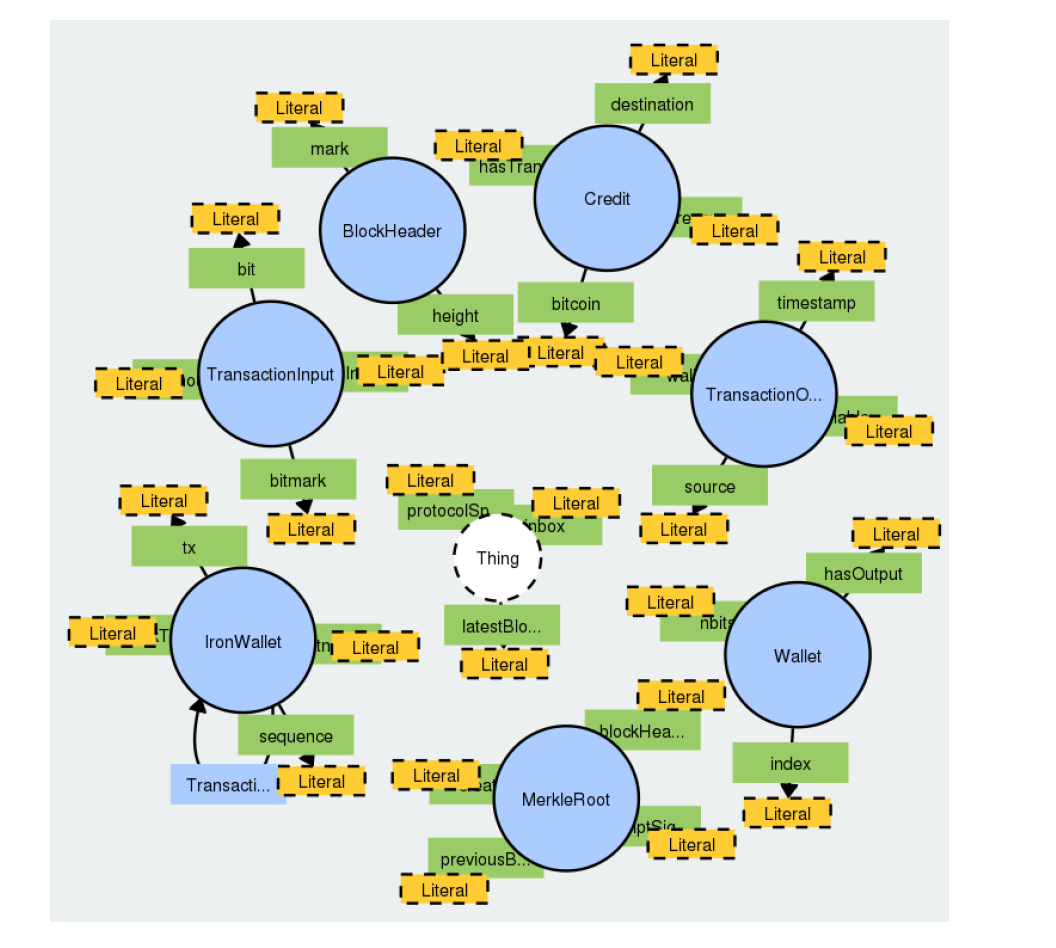
\includegraphics[width=1.65\textwidth]{images/chap02_diagram_ontology.png}
		\end{minipage}
		\caption[Illustration of Ontology diagram]{Illustration of Ontology diagram\cite{Matthew}}
		
		
	\end{figure}
	
\end{center}

\subsection{Linked Data}
Linked data is not a single format or standard but, as \textit{Tim Berbers-Lee} referred to in some informal documents is the \textit{expectation of behavior}. When information
is presented as Linked Data, other related information can be easily retrieved and new information also can be easily linked to it. \textit{Berners-Lee} described four rules for linked data:\\
\textbf{- URIs}(Uniform Resource identifier) as names.\\ 
\textbf{- HTTP} to search for names.\\
\textbf{- (SPARQL, RDF)}  when a user searches for something, provides related information.\\
\textbf{- Link} to other URLs to provide more information\cite{Hector}.\\

\begin{center}
	\begin{figure}[htb!]
		
		\begin{minipage}{0.55\linewidth}
			\centering
			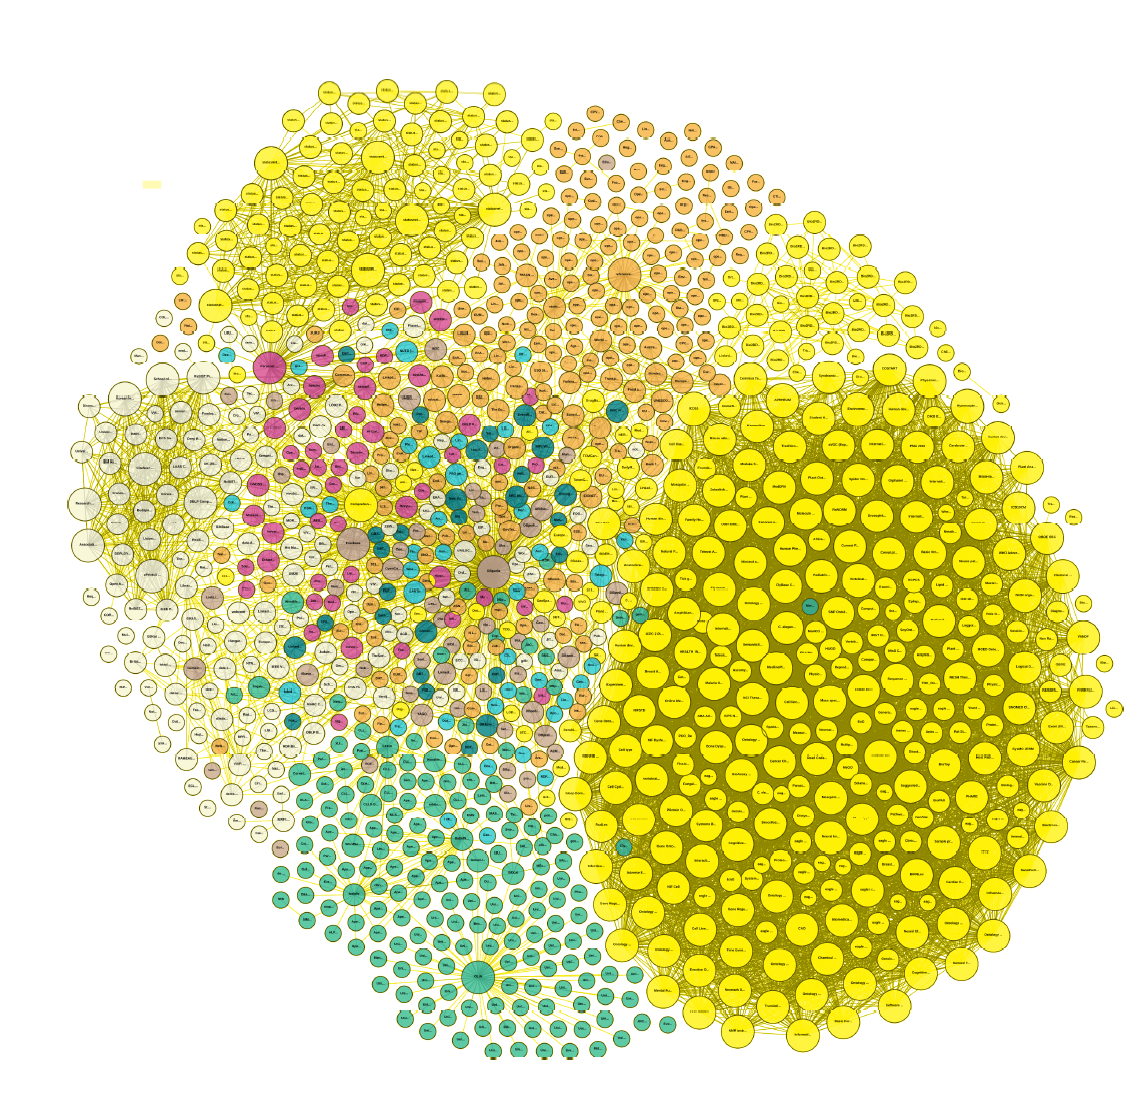
\includegraphics[width=1.55\textwidth]{images/chap02_LinkData.png}
		\end{minipage}
		\caption[Linked data diagram]{Linked data Diagram\cite{Hector}}
		
		
	\end{figure}
	
\end{center}
\subsection{RDF}
The Resource Description Framework (RDF) is a family
of W3C specifications. RDF is used to describe and model information. It describes a subject that predicts an object is called a triple.
i) Subjects that RDF expressions describe them.
ii) predict is specific properties, attributes, or relation to describe a resource.
iii) The object is the name of a property or value.
We can build a graph based on these three objects\cite{Hector}.

\subsection{SPARQL}
According to Wikipedia definition: It is a semantic query language for a dataset that makes us able to retrieve and modify data stored in RDF format known as triple. SPARQL can query the one, two, or all elements of triples.    

\subsection{Ontology Web Language }
Ontology Web Language is made to represent knowledge about things and the relations among them. OWL is a computational logic-based language, which means the language modeled in OWL can operate in a computer program like negation, intersection, and so on\cite{Hector}.

\subsection{Web 3.0}\cite{Hector}
Evolution and interaction of people on the Internet is classified based on three technologies:\\
\textit{Web 1.0} is known as \textit{web of document} is the earliest website with the basic capability of linking to other websites.\\
\textit{Web 2.0} known as  \textit{web of people} has the capability of providing space for users to collaborate with content creation or modification.\\
\textit{Web 3.0} is strengthened by the semantic web, where people have access to linked information on the web. But newly, with the arrival of distributed technology like blockchain, and Ethereum which get used by Web 3.0, this is a new focus on this.
\section{Vocabularies}
\subsection{Vocabulary in Distributed Ledger}
Generating linked data requires to use a standard ontology or vocabulary to explain the blockchain concepts. Interfaces between distributed ledgers and the Semantic Web are still in an early stage. Some systems define such vocabulary such as FlexLedger, EthOn, BLONDiE\cite{Third}.\\

\textbf{\textit{FlexLedger}}: describes HTTP interfaces to blockchains, with a standard vocabulary and responses of these interfaces. FLexLedger is a protocol for decentralized ledger and graph data model which represents ledger creation, querying, and data model using JSON-LD. However, FlexLedger does not have explicit vocabulary about ontology nor has concrete ontology for itself. \\
It is striking to say that the FlexLedger is not suitable to implement in some graph models like graph chain because in FlexLedger meta and the content data are stored together in the same graph whereas the GraphChain blocks’ content is stored outside the blockchain a separate graph \cite{Sopek}.\\

\textbf{\textit{EthOn}} is an OWl ontology that describes blockchain classes such as \textit{"blocks, accounts, message", "state"} and relations such \textit{"has parent block"}\cite{Rashid}. 
\begin{center}
	
	\begin{figure}[htb!]
		
		\begin{minipage}{0.50\linewidth}
			\centering
			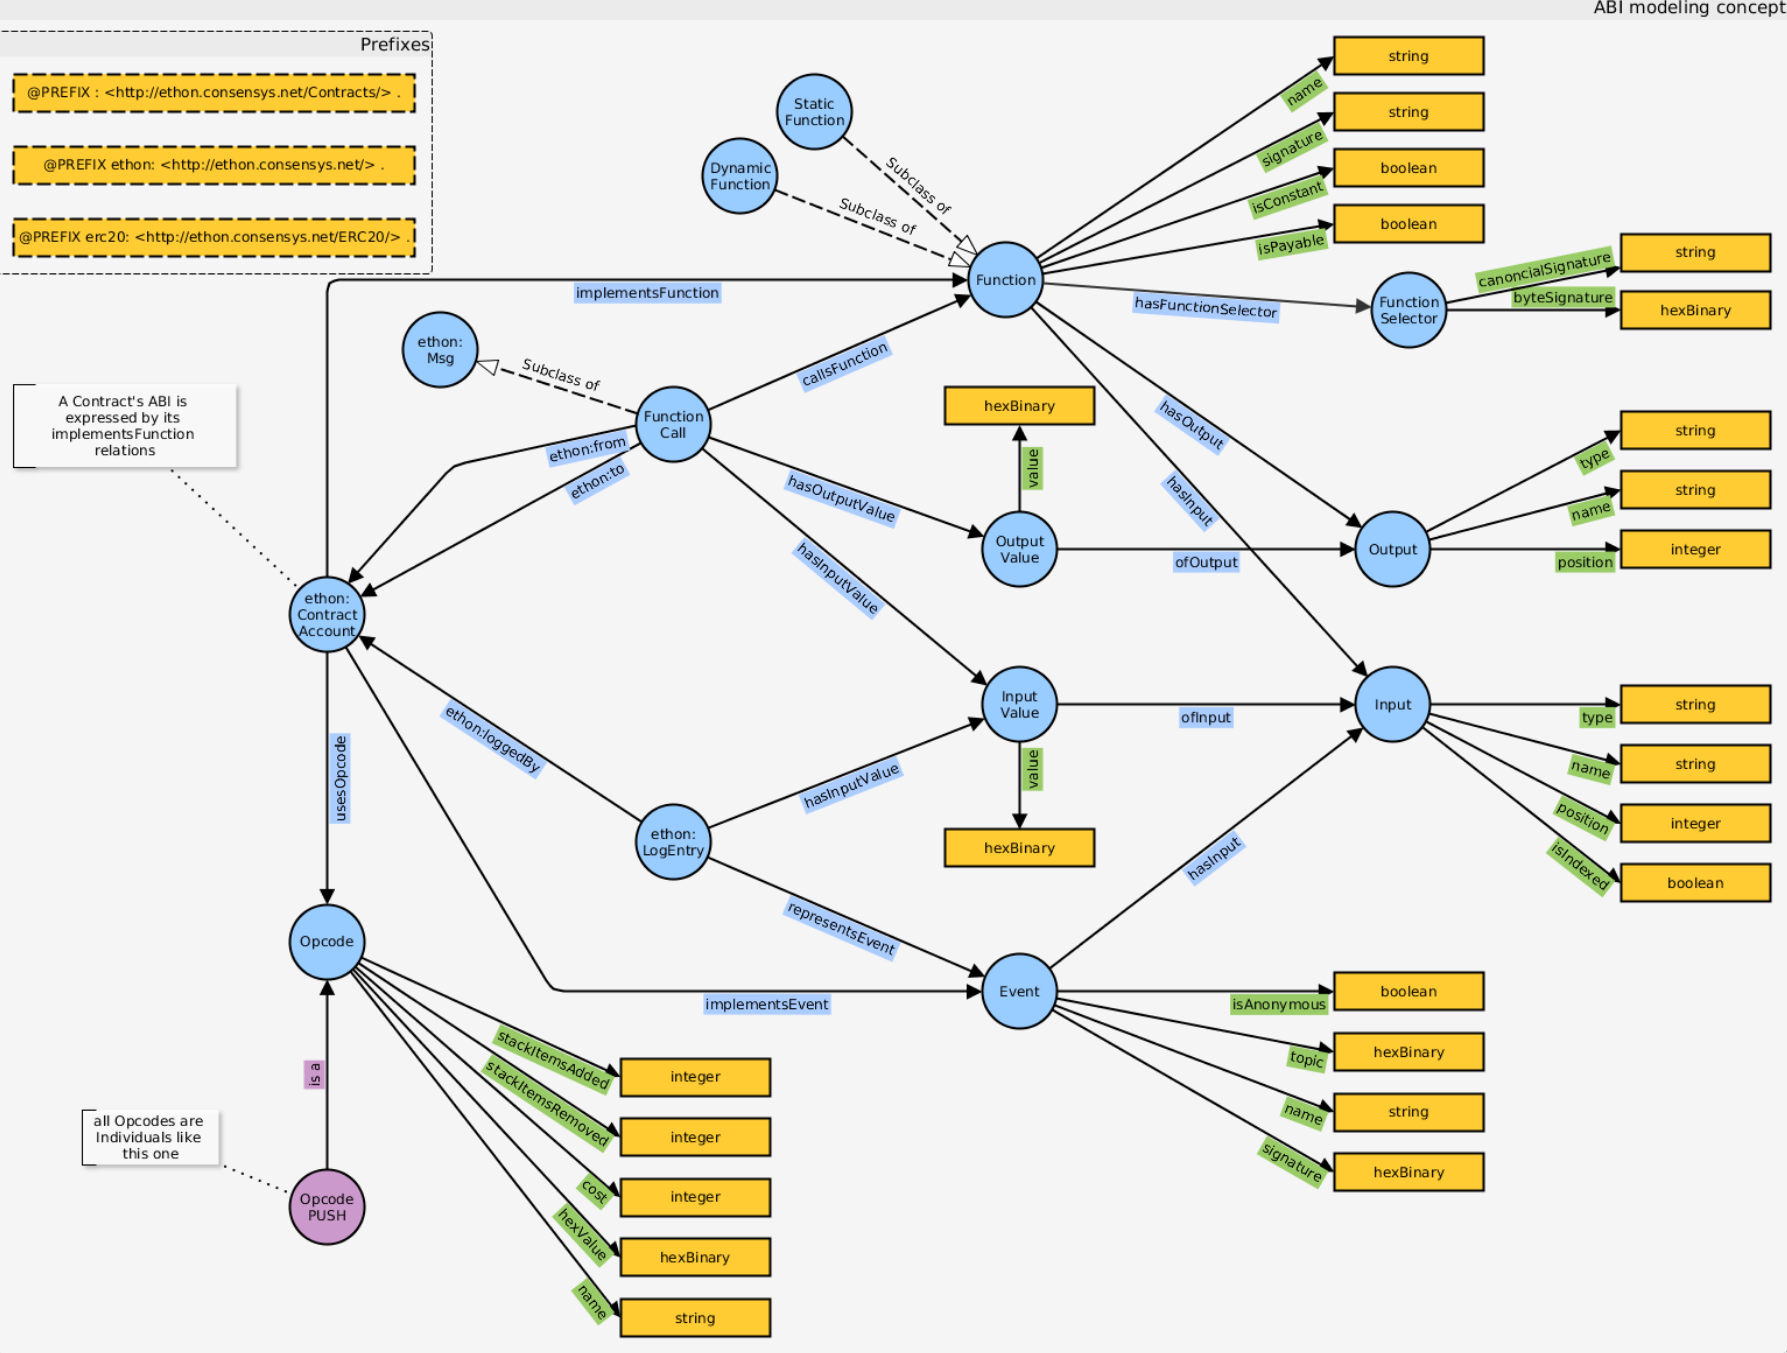
\includegraphics[width=1.80\textwidth]{images/chap2_EthOnContract.png}
		\end{minipage}
		\caption[EthOn classes]{EthOn Contract Model(blue arrow is object properties, green arrow is data properties, purple circle is instance and blue one is class)\cite{Rashid}}
		
	\end{figure}
	
	\begin{figure}[htb!]
		
		\begin{minipage}{0.55\linewidth}
			\centering
			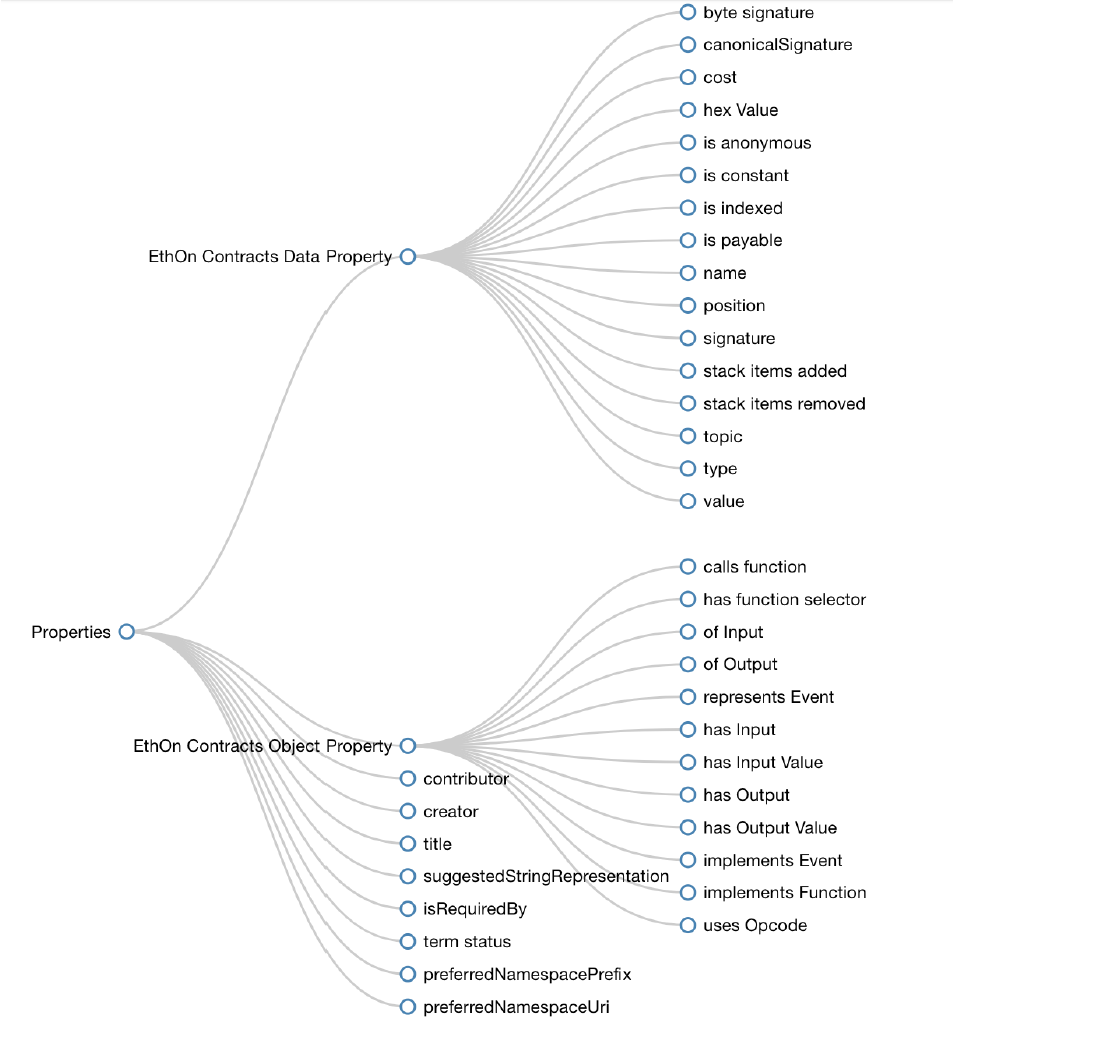
\includegraphics[width=1.65\textwidth]{images/chap02_EthOn_Properties.png}
		\end{minipage}
		\caption[EthOn Properties]{EthOn classes\cite{Rashid}}
		
		
	\end{figure}
	
\end{center}

\textbf{\textit{BLONDiE (Blockchain Ontology with Dynamic Extensibility)}} is another OWL ontology for describing the
Blockchain structure like EthOn. But, it is more generic than EthOn. For example, EthOn and BLONDiE both defined some terms such as 'account', 'block', and 'transaction', and some attributes such as 'transaction payload' or 'miner address'. BLONDiE defines some other concepts for different Blockchain such as 'BitcoinBlockHeader' and 'EthereumBlockHeader' as subclasses of 'BlockHeader'. At the moment, BLONDiE supports two cryptocurrencies like bitcoin and Ethereum where all links and relationships between objects and attributes represent in RDF(Resource Description Framework)\cite{Third}.
\begin{center}
	\begin{figure}[htb!]
		
		\begin{minipage}{0.55\linewidth}
			\centering
			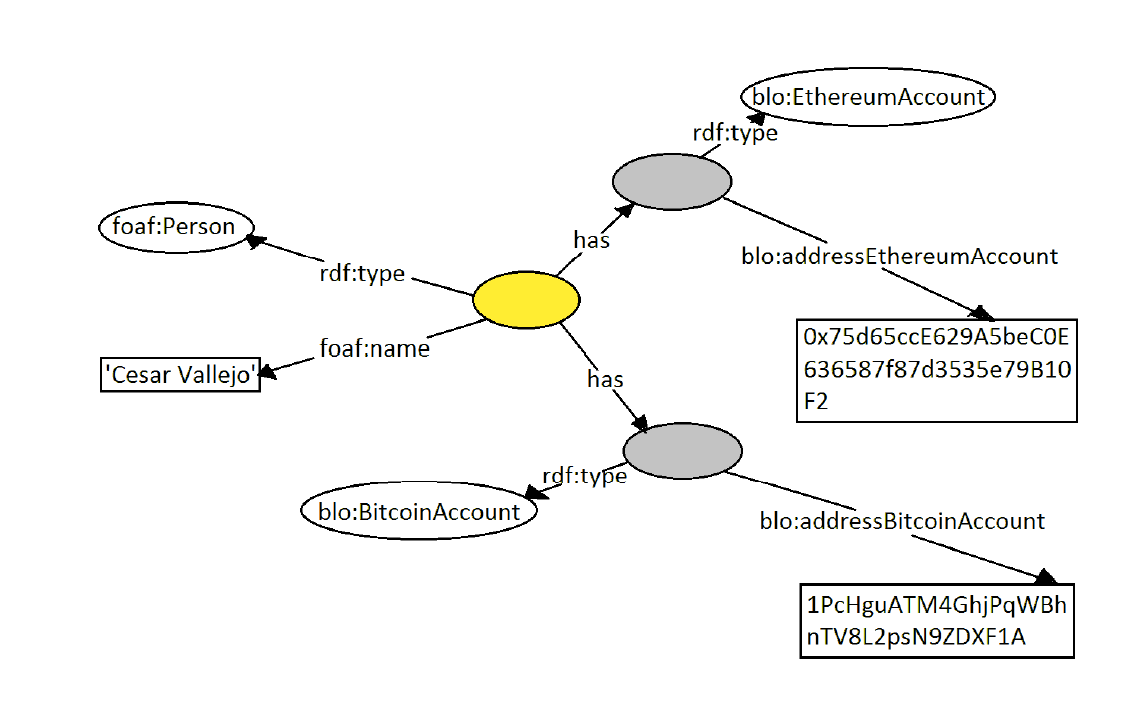
\includegraphics[width=1.75\textwidth]{images/chap02_BLONDiE.png}
		\end{minipage}
		\caption[BLONDiE]{BLONDiE usage example\cite{Hector}}
		
		
	\end{figure}
	
\end{center}
\subsection{Vocabulary in Smart Contracts}
As mentioned earlier, EthOn and BLONDiE are both similar concepts that can be used for smart contracts. As the smart contract is the executable software, the semantic and vocabulary apply to other software too.\\
There are many works on semantic annotation of the web and HTTP APIs which may enable us to annotate smart contracts as well. However, the contracts are not Web API and implementation may differ but the main concept does not differ. In other words, the vocabularies used to annotate web services, are used to annotate smart contracts too. It seems that the combination of a distributed ledger with the smart contract and web service due to profitability becomes common\cite{Third}.


\section{semantify Blockchain}
\subsection{Semantic Blockchain}
With increasing the usage of blockchain technology recently, the need for semantic reasoning on the distributed ledger is on the crease as well. The blockchain is the best platform to utilize semantic web principles in this technology and add a new trusted property to a dataset. It makes a new dataset so trustworthy. 
Using semantic web technology on the blockchain is a novel idea and the way how to apply this technology in blockchain and smart contracts is also a controversial issue.\\
There are some \textbf{definition of semantic blockchain:}\\ 
\textit{- Semantic blockchain is the representation of stored data on distributed ledger using linked data. }\\
\textit{- Semantic blockchain is the applying semantic web standard on the blockchain that these standards are based on RDF.}

\subsection{Semantification process}
Semantic blockchain or semantic distributed ledger affects the industrial world and subsequently, the result leads to start development new application and frameworks to combine two worlds:
these are some ways to sanctify blockchain:\\
\textbf{-}Mapping the blockchain data to RDF making usage of vocabulary, ontology, and so on.\\
\textbf{-} Storage of data in a blockchain is expensive, The only way is to store the hashing point to the data set in the blockchain and then share RDF on the blockchain. \\
\textbf{-} Create semantic blockchain that internal data exchange protocol in RDF format\cite{Hector}. \\

\subsection{Semantic Ontology Mapping using BLONDiE} 
To generate RDF, it needs to map the basic blockchain entities to relevant semantic web terms, concepts, and ontology. To make the query more efficient, BLONDiE used some ways such as \\  
Firstly, records relating to both block and transactions have been
augmented with an attribute for the hash of each entity,   \\
Secondly, records relating to the transactions have been augmented with links to entities like blocks or smart contracts.\\
Blockchain stores just a binary form of each contract with metadata.   
To interact with the contract Application Binary(ABI) Interface specification is required. This specification is in the form of JSON and is created when a smart contract is compiled and stored in the blockchain. The ABI determines all functions of contracts and descriptions about input, and output parameter for each contract\cite{Third}.

\begin{center}
	\begin{figure}[htb!]
		
		\begin{minipage}{0.55\linewidth}
			\centering
			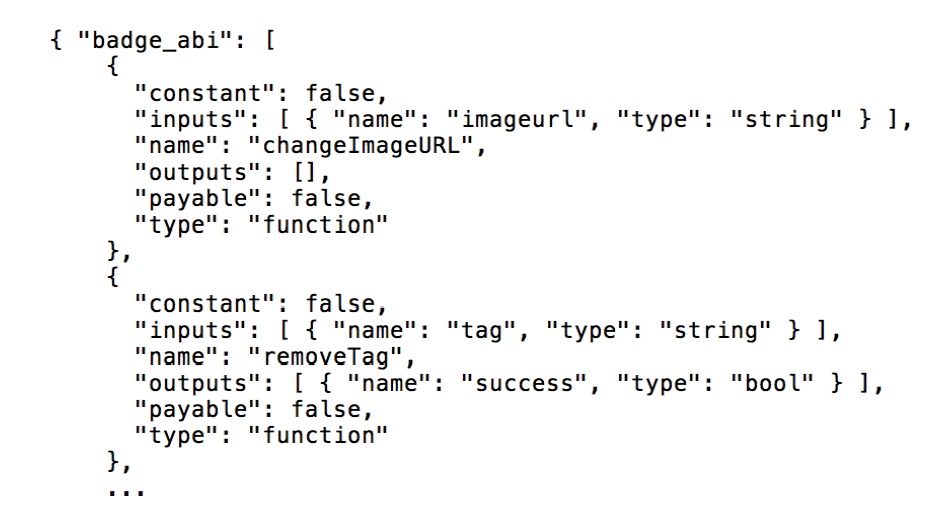
\includegraphics[width=1.95\textwidth]{images/chap02_SmartContract_ABI.png}
		\end{minipage}
		\caption[Smart contract of ABI]{Smart  contract of ABI}
		
	\end{figure}
	
\end{center}



